\documentclass[11pt,a4paper]{report} 
% Alternativ für doppelseitigen Ausdruck (nur bei > 60 Seiten sinnvoll)
% \documentclass[11pt,a4paper,twoside,openright]{report} 
\usepackage{mathtools}
\usepackage{amssymb} 

% Deutsch
%\usepackage[german]{babel} % deutsch und deutsche Rechtschreibung
%\usepackage[english]{babel}
\usepackage[main=english, german]{babel}
\usepackage[utf8]{inputenc} % Unicode Text 
\usepackage[T1]{fontenc} % Umlaute und deutsches Trennen
\usepackage{textcomp} % Euro
\usepackage[hyphens]{url}
% statt immer Ab\-schluss\-ar\-beit zu schreiben
% einfach hier sammeln mit -. 
\hyphenation{Ab-schluss-ar-beit}
% Vorsicht bei Umlauten und Bindestrichen
\hyphenation{Ver-st\"ar-ker-aus-gang}
 % eigene Hyphenations, die für das Dokument gelten
\usepackage{amssymb} % Symbole
\usepackage{emptypage} % Wirklich leer bei leeren Seiten


%% Fonts, ein kompletter Satz an Optionen

% Times New Roman, gewohnter Font, ok tt und serifenlos
%\usepackage{mathptmx} 
%\usepackage[scaled=.95]{helvet}
%\usepackage{courier}

% Palatino mit guten Fonts für tt und serifenlos
\usepackage{mathpazo} % Palatino, mal was anderes
\usepackage[scaled=.95]{helvet}
\usepackage{courier}

% New Century Schoolbook sieht auch nett aus (macht auch tt und serifenlos)
%\usepackage{newcent}

% Oder default serifenlos mit Helvetica 
% ich kann es nicht mehr sehen ...
%\renewcommand{\familydefault}{\sfdefault}

\usepackage{microtype}

% Bilder und Listings
\usepackage{graphicx} % wir wollen Bilder einfügen
\usepackage{subfig} % Teilbilder
\usepackage{wrapfig} % vielleicht doch besser vermeiden
\usepackage{listings} % schöne Quellcode-Listings
% ein paar Einstellungen für akzeptable Listings
\lstset{basicstyle=\ttfamily, columns=[l]flexible, mathescape=true, showstringspaces=false, numbers=left, numberstyle=\tiny}
\lstset{language=python} % und nur schöne Programmiersprachen ;-)
% und eine eigene Umgebung für Listings
\usepackage{float}
\newfloat{listing}{htbp}{scl}[chapter]
\floatname{listing}{Listing}

% Seitenlayout
\usepackage[paper=a4paper,width=14cm,left=35mm,height=22cm]{geometry}
\usepackage{setspace}
\linespread{1.15}
\setlength{\parskip}{0.5em}
\setlength{\parindent}{0em} % im Deutschen Einrückung nicht üblich, leider

% Seitenmarkierungen 
\newcommand{\phv}{\fontfamily{phv}\fontseries{m}\fontsize{9}{11}\selectfont}
\usepackage{fancyhdr} % Schickere Header und Footer
\pagestyle{fancy}
\renewcommand{\chaptermark}[1]{\markboth{#1}{}}
%\fancyhead[L]{\phv \leftmark}
\fancyhead[L]{\phv \nouppercase{\leftmark}}
\fancyhead[R]{\phv \thepage}
% Unten besser auf alles Verzichten
%\fancyfoot[L]{\textsf{\small \kurztitel}}
\fancyfoot[C]{\ } % keine Seitenzahl unten
%\fancyfoot[R]{\textsf{\small Medieninformatik}}

% Theorem-Umgebungen
\newtheorem{definition}{Definition}[chapter]
\newtheorem{satz}{Satz}[chapter]
\newtheorem{lemma}[satz]{Lemma} % gleicher Zähler wie Satz
\newtheorem{theorem}{Theorem}[chapter]
\newenvironment{beweis}[1][Beweis]{\begin{trivlist}
\item[\hskip \labelsep {\textit{#1 }}]}{\end{trivlist}}
\newcommand{\qed}{\hfill \ensuremath{\square}}

% Quellen teilen
\usepackage{bibtopic} 

% Hochschule Logo, noch nicht perfekt
\usepackage{hsrmlogo}

% Spezialpakete
\usepackage{epigraph}
\setlength{\epigraphrule}{0pt} % kein Trennstrich

% damit wir nicht so viel tippen müssen, nur für Demo 
\usepackage{blindtext} 

% Zum Zeigen von Fehlern
\usepackage{soul}
\newcommand*\falsch{\st}

 % alle Pakete und Einstellungen

% Hier anpassen 
\newcommand{\welchethesis}{Bachelor}
% \newcommand{\welchethesis}{Master}
\newcommand{\thesisofwas}{of Science - B.Sc.}
\newcommand{\titel}{Study and implementation of a decentralized application that can provide
	permissionless financial services using an evm based blockchain}
%\newcommand{\kurztitel}{Template Abschlussarbeit}
\newcommand{\autor}{Mario Alberto Maita Orozco}
\newcommand{\datum}{30.06.2022} % Abgabedatum
\newcommand{\ort}{Wiesbaden}
\newcommand{\referent}{Prof.\ Dr.\ Eva-Maria Iwer}
\newcommand{\korreferent}{Prof.\ Dr.\ Marc-Alexander Zschiegner}
%\usepackage{tabularx}
\usepackage{enumitem}
\usepackage{hyperref}
\hypersetup{
	colorlinks=true,
	linkcolor=blue,
	filecolor=magenta,      
	urlcolor=cyan,
	citecolor=blue,
%	pdftitle={Overleaf Example},
%	pdfpagemode=FullScreen,
}
\begin{document}

\begin{titlepage}
  \begin{center}
    % Kopf der Seite
    \hsrmlogo[1]
    \parbox[b]{8cm}{Hochschule RheinMain \\
     Fachbereich Design Informatik Medien \\
     Studiengang Informatik - Technische Systeme}
    \vfill    
    {\LARGE Bachelor-Arbeit} \\[0.5cm]
    {\large zur Erlangung des akademischen Grades} \\[5mm]
    {\large \welchethesis\ \thesisofwas} \\[5mm]
    \rule{\textwidth}{1pt}\\[0.5cm]
    {\begin{spacing}{1.15} \LARGE \bfseries \titel \\ \end{spacing}}
    \rule{\textwidth}{1pt}    
    \vfill    
    \begin{tabular}{ll} % Mitte der Seite
      Vorgelegt von & \autor \\
      am & \datum \\
      Referent & \referent \\
      Korreferent & \korreferent
    \end{tabular}    
    \vfill
  \end{center}
\end{titlepage}
\cleardoublepage


% Erklärung gemäß den Allgemeinen Bestimmungen für Prüfungsordnungen
% der Paragraph schwankt, daher ohne Nennung einer Nummer
\thispagestyle{empty}
\section*{Erklärung gem. ABPO, Ziff. 4.1.5.4}
Ich versichere, dass ich die Bachelor-Arbeit selbständig verfasst und keine anderen als
die angegebenen Hilfsmittel benutzt habe.
´

\vspace{6em}
\noindent\begin{tabular}{p{0.37\textwidth}p{0.56\textwidth}}
\ort, \datum  & \rule{0.56\textwidth}{0.5pt}\\
              & \makebox[1cm]{\ } \autor
\end{tabular}

\vfill

\section*{Erklärung zur Verwendung der \welchethesis thesis}

Hiermit erkläre ich mein Einverständnis mit den im Folgenden aufgeführten
Verbreitungsformen dieser Bachelor-Arbeit:

\vspace{1em}
\noindent\begin{tabular}{|p{0.82\textwidth}|c|c|}
  \hline
  \textbf{Verbreitungsform} & \makebox[0.035\textwidth]{\textbf{Ja}} 
                            & \makebox[0.05\textwidth]{\textbf{Nein}} \\\hline
  Einstellung der Arbeit in die Hochschulbibliothek 
                         mit Datenträger   &  & $\times$ \\\hline
  Einstellung der Arbeit in die Hochschulbibliothek  
                         ohne Datenträger  & $\times$ & \\\hline
  Veröffentlichung des Titels der Arbeit im Internet  
                                           & $\times$ & \\\hline
  Veröffentlichung der Arbeit im Internet             
                                           &  $\times$  & \\\hline
\end{tabular}

\vspace{6em}
\noindent\begin{tabular}{p{0.37\textwidth}p{0.56\textwidth}}
\ort, \datum  & \rule{0.56\textwidth}{0.5pt}\\
              & \makebox[1cm]{\ } \autor
\end{tabular}
\cleardoublepage

 % Titelseite, Erklärungen, etc.

\begin{abstract} 
abstract
\end{abstract}

\tableofcontents
\newpage 

\chapter{Introduction} \label{ch:intro}
%\epigraphhead[70]{\epigraph{Documentation is like sex: 
%when it is good, it is very, very good; and when it is bad, 
%sit is better than nothing.}{\textit{Dick Brandon}}}



\section{Motivation}
In the last years' blockchain technology has gained a lot of traction and many developers are willing to build applications on top of this technology.
The Ethereum network with the Ethereum Virtual Machine, or EVM~\ref{sec:evm}, (whose state is validated and copied by every node of the network) offers a new way of application development. Meaning that developers can now implement some functionality and deploy it to a public EVM blockchain, making the code/functionality tamper-resistant; in addition, the implemented functionality (or smart contract) can be called by any participant or other code/contracts within the network. This composability allows anyone to interact with already deployed contracts and build other applications on top of them. 
These kinds of applications are called Decentralized applications or Dapps~\ref{sec:dapps}, because they are built on top of a decentralized network such as  Ethereum.
\section{Goals}
The goals of this Thesis are, to study and provide a better understanding of: 
\begin{itemize}
	\item How Dapps are built.
	\item Which technology is used.
	\item And the development of a Dapp that uses well-known DeFi protocols ~\ref{ch:defi}, to let users access to permissionless financial services such as lending and borrowing of crypto assets.
\end{itemize}


\section{Thesis Structure}
The Thesis is divided into the following chapters:
\begin{itemize}
	
	\item \textbf{Chapter ~\ref{ch:background} - Fundamentals}, gives a technical overwiev of the blockchain technology and the Ethereum network.
	\item \textbf{Chapter ~\ref{ch:defi}} ...
	\item \textbf{Chapter ~\ref{ch:appreq}} ...
	\item \textbf{Chapter ~\ref{ch:impl}} ...
	\item \textbf{Chapter ~\ref{ch:conclusion}} ...
\end{itemize}


%%%%%
%%%%% Chapter
\chapter{Fundamentals} \label{ch:background}

\section{Blockchain} \label{sec:bc}
A blockchain\cite{book:bc}\cite{article:bc} is a type of database (append-only data strucuture), which stores data in blocks. These blocks are chronologically ordered by discrete timestamps and linked to each other using cryptographic hash functions\cite{chf}\cite{book:chf}. Commonly, a blockchain is used as a public distributed ledger of transactions records, shared and synchronized by a per-to-per network~\ref{subsec:p2p}, where every party can participate in the validation of new blocks based on a consensus protocol, see~\ref{sec:cp}.
The idea of a cryptographically secured chain of blocks was originally presented by Haber and Stornetta\cite{time-stamp} in 1991. However, the implementation and adoption of this technology started with the conception of the bitcoin cryptocurrency whitepaper\cite{bitcoin} in 2008.

\begin{figure}[htp]
	\centering
	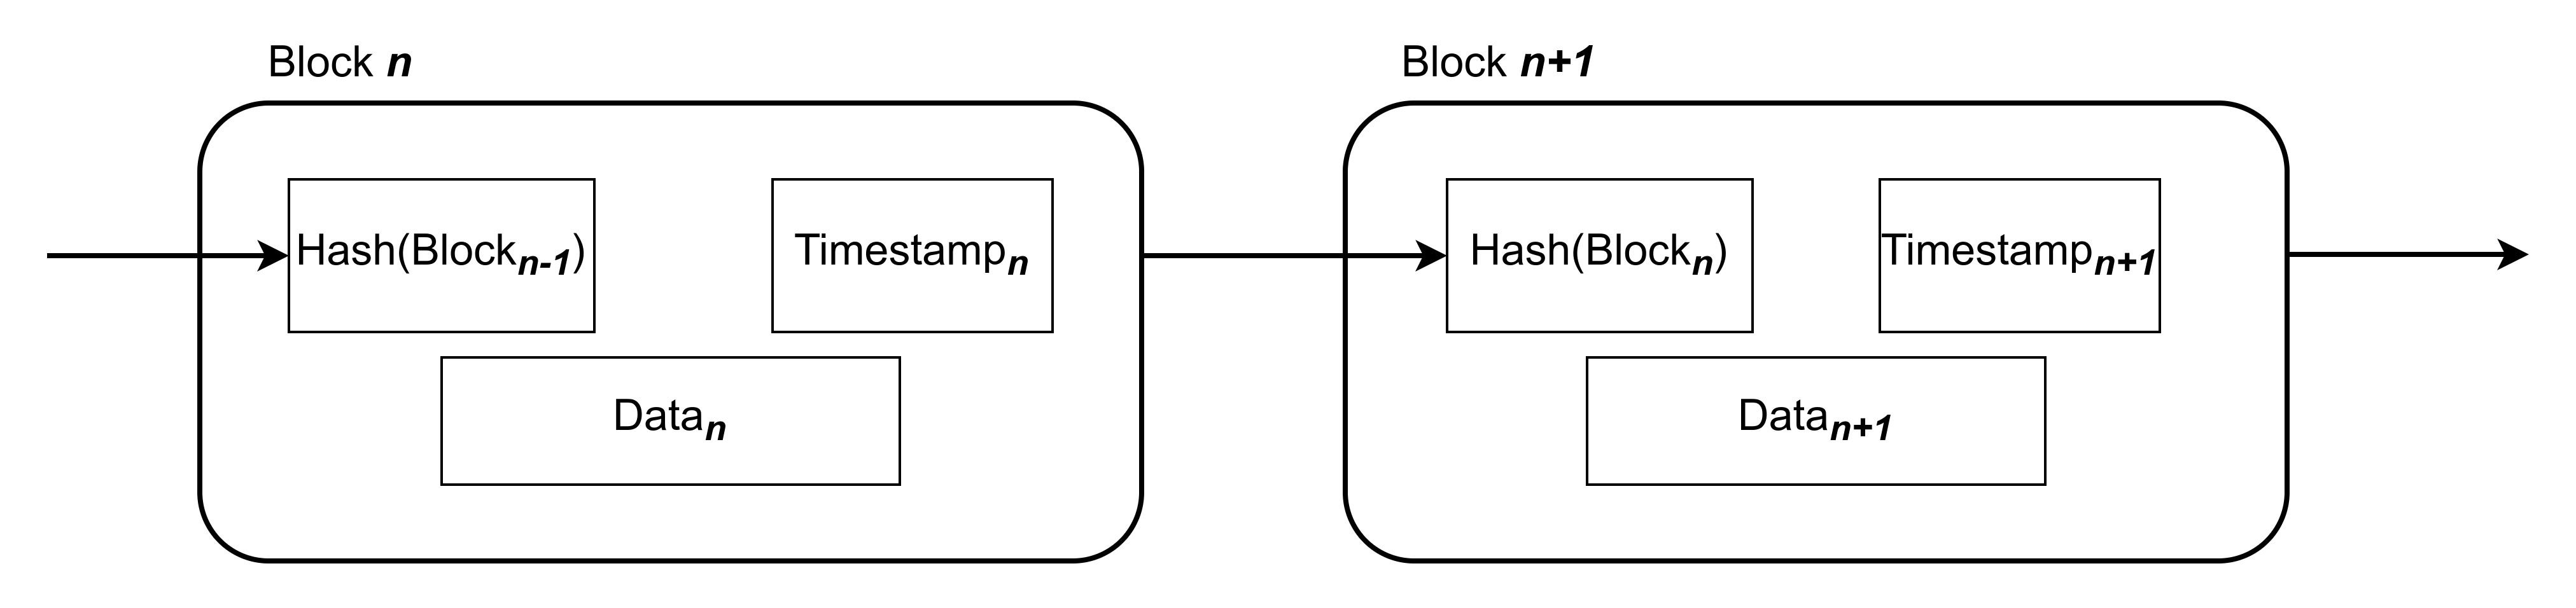
\includegraphics[width=1\textwidth]{./images/bc}
	\caption{View of two blocks in a blockchain}
	\label{fig:bc}
\end{figure}

Determined by the blockchain implementation, block contents can be different. A block usually has a timestamp, the data or transactions record, and the hash value of the previous block in the chain, see figure~\ref{fig:bc}.
The way that a blockchain ensures the security and keeps the integrity of the data is through cryptographic hash functions \ref{sec:chf}, and Merkle trees \ref{sec:mt}

By adding the cryptographic hash value of the previous block  (Block $n$ to Block $n+1$), blockchains ensure the integrity of previous blocks. Because of the second preimage resistance of cryptographic hash functions, see~\ref{sec:chf}, it is computationally infeasible to  find an input other then Block $n$ in order to generate an output = Hash (Block $n$). Due to that, the further the blockchain grows beyond block $n$, the more secure is the integrity of block $n$ and previous blocks.

Depending on who can participate in the consensus protocol, blockchain networks can be divided into two groups: permissionless and permissioned blockchains. This Thesis will be focused on permissionless blockchains that use an EVM, such as the Ethereum network.

\subsubsection{Peer-to-peer (P2P) network}\label{subsec:p2p}
\begin{figure}[htp]
	\centering
	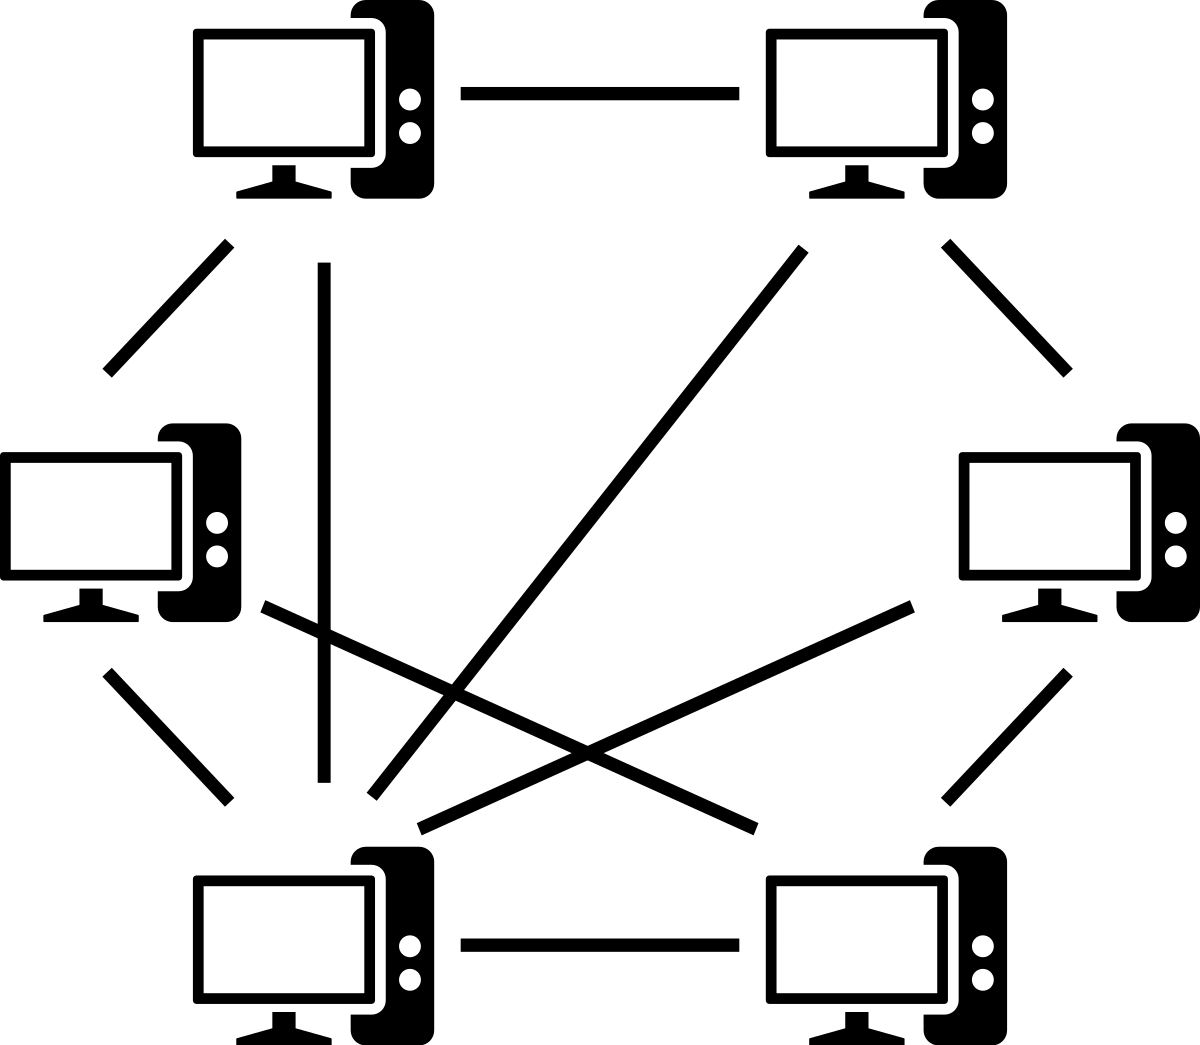
\includegraphics[width=0.45\textwidth]{./images/p2p}
	\caption{Peer-to-peer network\cite{wiki:Peer-to-peer}}
	\label{fig:p2p}
\end{figure}
A peer-to-peer network\cite{book:masteringBTCp2p}\cite{wiki:Peer-to-peer} is a decentralized communications model where each participant (node) of the network stores and shares data with other nodes without any central party. Every peer is equal and there is no special node. Due to the decentralized design, P2P networks are resilient and robust compared with typical client-server architecture. The distributed ledger or blockchain is managed by the peer-to-peer network based on a set of rules or consensus mechanisms~\ref{sec:cp}, in fact, the term \emph{blockchain network} refers to a set of nodes, of a peer-to-peer network, running the consensus protocol of the specific blockchain. 



\subsection{Cryptographic hash functions}\label{sec:chf}
A cryptographic hash function\cite{chf}\cite{book:chf} maps a given data of variable size to a fixed length \emph{n}-bit string called hash value. $ H : \{0,1\}^* \to \{0,1\}^n $ Such hash functions have the following properties:
\begin{description}		
	\item \textbf{Collision resistance}: Given $x_1, x_2 $ It should be necessary $ O(2^\frac{n}{2}) $ compute power such that $H(x_1) = H(x_2).$This means, that it will be computationally infeasible that different inputs, i.e., blocks of data, will generate the same hash value.	
	\item \textbf{Preimage resistance}: For a hash value \emph{h}, it should be necessary $ O(2^n) $ computation power in order to obtain an \emph{x} such that $ H(x)=h $.~~In other words, it should be a one-way function. 
	This means that it is computationally infeasible to retrieve the input data from its hash value. For instance, it is nearly impossible to get a private key from its public key.	
	\item \textbf{Second preimage resistance}: For an input $x_1$ and its hash value $h_1$, it should be necessary $ O(2^n) $ computation power in order to obtain a $x_2$ such that $H(x_2)=h_1.$ This means that for a given hash value, it is computationally infeasible to find another input, i.e., a block data input, that generates the same hash value. 	
\end{description}

Such properties prevent attackers from modifying existing blocks keeping the blockchain intact. For example, the bitcoin network uses the SHA-256 hashing algorithm to validate a block, and append it to the chain. This means once a consensus among all the participants is done, and a new block is added, it will be required $ O(2^{256}) $ computation power to tamper with the blockchain. In other words, it is nearly impossible to manipulate an added block as a result of the tremendous computer power that would be needed.

\subsection{Merkle tree}\label{sec:mt}
A Merkle tree\cite{article:merkle}\cite{book:merkle} or hash tree is a binary tree where every leaf node (nodes at the bottom of the tree) is the cryptographic hash value of some data or transaction. A merkle tree is constructed bottom-up; the upwards nodes are the cryptographic hash values of its two child nodes. Therefore, the root node  will contain a complete fingerprint of the entire set of transactions. 

Merkle trees allow secure and efficient data verification using cryptographic hash functions. For example; if a participant in the network needs to verify the validity of these four transactions, see figure~\ref{fig:merkle}, only a check of the root hash value is necessary. Due to the Merkle tree structure, if any of the data blocks is modified, so will be the root hash value. Furthermore, Merkle tree is a very efficient data structure; for instance, checking that a given transaction is included in the tree will take a maximum of $2log (N)$ operations.
\begin{figure}[htp]
	\centering
	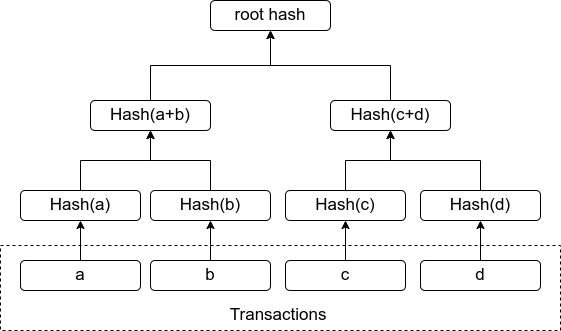
\includegraphics[width=0.65\textwidth]{./images/merkle}
	\caption{Merkle tree of four transactions}
	\label{fig:merkle}
\end{figure}
\subsection{Consensus Protocol}\label{sec:cp}
The consensus protocol\cite{article:bc} of a blockchain network gives a specific rule for verifying whether a transaction is valid or not. As mentioned in~\ref{sec:bc}, any participant or node of the network, depending on the blockchain type, can append a new block. For the reason that blockchains typically do not have a centralized authority validating transactions, participants on the blockchain must verify any transaction according to the set of rules or consensus protocol of the blockchain. The most common consensus mechanisms nowadays are:
\begin{itemize}
	\item[] \textbf{Proof of work (PoW)}
	In a PoW blockchain, nodes have to solve a cryptographic task in order to validate a block, the first node to find a solution can submit the transaction. Most of the first blockchains in the space use proof-of-work-based protocols; for example, Bitcoin uses PoW based on the cryptographic hash function SHA-256.	
	\item[] \textbf{Proof of state (PoS)}
	In a PoS blockchain, the entity that can validate a transaction is randomly selected, depending on the "stake" that a node has on the network. Since nodes have a large stake in the blockchain, they will pursue the integrity of the network.

\end{itemize}
\subsection{Public-Key Cryptography}
In order to interact with a blockchain, participants use public key cryptography or asymmetric key cryptography\cite{book:pkc}. The public key acts as the id of the sender or receiver of a given message; and it can be shared with others without any security downfall. On the other hand, the private key should be kept secure and private by the message sender; it is used to sign (digital signature) the messages or transactions, i.e., give permission to change the state of the user records in the blockchain.
\begin{itemize}
	\item[] \textbf{Digital signature:} The message or transaction can only be signed with a private key, and anyone who knows the public key of the signed message can verify  its authenticity. Meaning that any party of the blockchain can participate in the verification of the transactions/messages.
\end{itemize}
The private key is a random number and the public key is generated from it using one-way cryptographic hash functions, see \ref{sec:chf} or elliptic curve cryptography\cite{book:pkc}\cite{wiki:ecc}. Elliptic curve cryptography (ECC) is based on the discrete logarithm problem and is the most common public-key algorithm in blockchain networks.
In mathematics terms, an elliptic curve is a plane curve over all the points $(x, y)$ that satisfy the following equation:  $ y^2 = x^3 +ax + b $

%\subsection{Bitcoin}
%The bitcoin network is a set of technologies that enabled for the first time a %decentralized, permissionless, trustless, peer-to-peer digital currency system. %The distributed computation system that bitcoin introduced: the proof-of-work %algorithm to produce a consensus in a distributed system without a central %trusted authority, in combination with the blockchain storage system, solved the %double-spend problem and the Byzantine generals problem.

\section{Ethereum}\label{sec:eth}
The Bitcoin\cite{bitcoin}\cite{book:masteringBTC} network and its set of technologies enabled for the first time a decentralized, permissionless, trustless, peer-to-peer digital currency system. The distributed computation system that bitcoin introduced: a proof-of-work algorithm to produce a consensus in a distributed system without a central trusted authority, in combination with the blockchain storage system, solved the double-spend problem and the Byzantine generals problem, enabling other applicability beyond digital currencies.  In 2014, Vitalik Butering introduced Ethereum\cite{article:eth}, a platform that moved beyond cryptocurrency applications.

Similar to Bitcoin, Ethereum\cite{article:eth}\cite{book:masteringETH} is a distributed transaction-based state machine. However, it is not only a cryptocurrency system. Ethereum is a decentralized computing platform or a decentralized, pseudo-turning complete virtual machine, which runs smart contracts and stores its state changes in its blockchain. Like bitcoin, state changes in ethereum are managed by a consensus mechanism, where everyone can participate in the validation of  blocks or state changes.

\subsection{Accounts}\label{sec:accounts}
Ethereum\cite{article:eth}\cite{wood2014ethereum} has an account-based model, where every account represents a state. An account is mapped with a 160 bits address (public key) and there are two types of accounts: \textit{Externally owned account} (EOA), controlled by a private key and (smart) \textit{contract account}, controlled by EVM code. Depending on the account type, an account state is represented by the following four fields: \textbf{Nonce} is a counter that represents the number of transactions or contracts created by the account. \textbf{Balance} is the amount of Ether owned by the account, expressed in Wei~\ref{tab:Ether_metrics}. \textbf{Storage hash} is the root hash of a merkle tree that represents the contents of the account. \textbf{Code hash} is the hash that points to the EVM code that the account has.
\begin{figure}[htp]
	\centering
	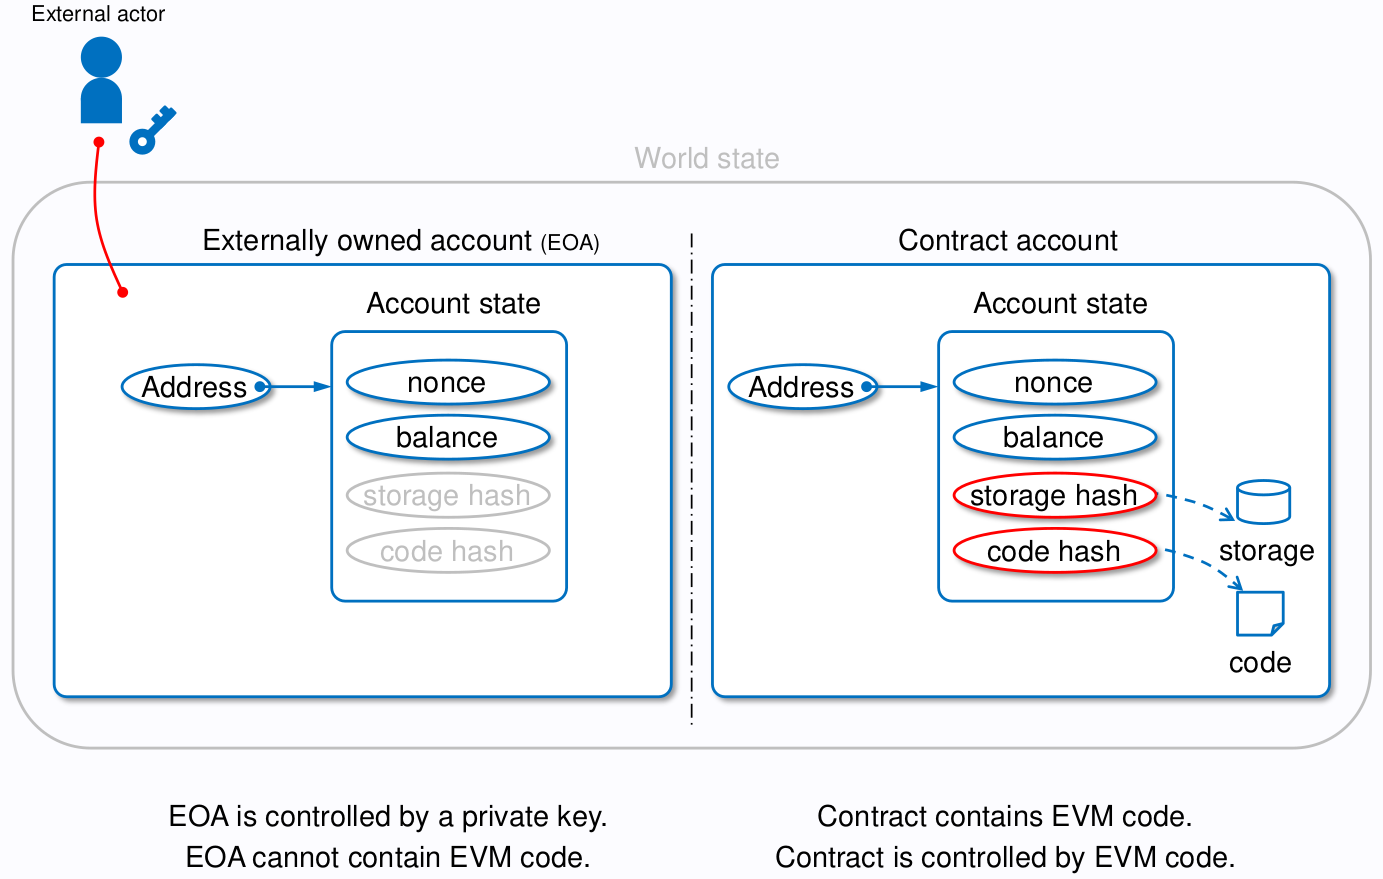
\includegraphics[width=0.8\textwidth]{./images/accounts}
	\caption{Ethereum Accounts\cite{evm-illustrate}}
	\label{fig:accounts}
\end{figure}

\subsubsection{Transactions and Messages}
A \textbf{transaction} is a cryptographically-signed message that can only be sent by an EOA. Transactions can trigger a state change on the blockchain or the execution of EVM code. Transactions can be divided into two groups:
\begin{itemize}
	\item  \textbf{Message calls}: The transactions between accounts.
	\item \textbf{Contract creations}: creation of a new account with EVM code in its data/code field.
\end{itemize}
\textbf{Messages} can be seen as internal transactions between contracts triggered by a message call. A message is like a transaction but produced by a contract. This way messages enable contracts to interact between them.
\subsection{Ethereum Virtual Machine (EVM)}\label{sec:evm}
The EVM\cite{wood2014ethereum}\cite{book:masteringETH-evm} is a quasi-Turing-complete machine; the quasi means that its computation is limited by the available \textbf{gas}~\ref{sec:gas} that the executed contract bytecode has, preventing that accidentally or malicious contracts execute forever. Thus, denial-of-service attacks are not possible on Ethereum. The EVM is a stack machine with 1024 elements. It is big-endian by design with 256-bit word size, which facilitates hashing and elliptic curve operations (Keccak-256 hashes and secp256k1 signatures). In addition to the {\textbf{Stack}}, the machine has two more  spaces where operations can access and store data: {\textbf{Memory}}; volatile and initialized to zero. \textbf{Account storage}; non-volatile and maintained as part of the Ethereum state, also initialized to zero. Lastly, the EVM code is stored in a separate virtual read-only memory (\textbf{ROM}).
\begin{figure}[htp]
	\centering
	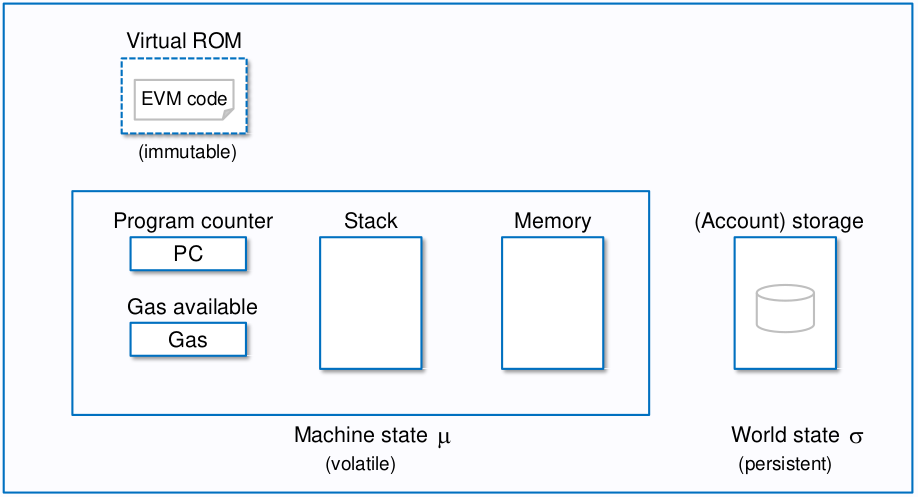
\includegraphics[width=0.65\textwidth]{./images/evm}
	\caption{Ethereum Virtual Machine\cite{evm-illustrate}}
	\label{fig:accounts}
\end{figure}
\subsubsection{Ether and Gas}\label{sec:gas}
Ether (ETH) is the native cryptocurrency of Ethereum. Ether is used to pay for transaction fees or EVM computing power in the form of gas units. For example, the cost or gas limit for sending a transaction is 21000 gas units\cite{wood2014ethereum-Fee}. The price for a gas unit is represented in gwei, and is set by the participants of the consensus protocol (miners), based on the supply and demand of the network computational power\cite{book:masteringETH-gas}.
For instance, with an average gas price of 15 gwei\cite{gastracker}, sending a transaction at the moment of writing this Thesis would cost: $21000*15 = 315000~Gwei$ or $0.000315~Ether.$
\begin{table}[htp]
\centering
%\begin{center}
\begin{tabular}{|l|l|l|}
	\hline
	\multicolumn{1}{|c|}{\textbf{Unit Name}} & 
	\multicolumn{1}{|c|}{\textbf{Wei Value}} \\\hline
	$Ether$ & $1^{18}$  \\\hline
	$Gwei$  & $1^{9}$  \\\hline
	$Wei$   & $1$     \\\hline   
\end{tabular}
\caption{Important metrics of $Ether$}
\label{tab:Ether_metrics}
%\end{center}
\end{table}

\subsection{Smart Contracts}\label{sec:sc}
In the Ethereum network, a smart contract\cite{book:masteringETH-sc-solidity}\cite{smartcontracts} is a computer program that is executed by the EVM. Since smart contacts are also a type of account, see~\ref{sec:accounts}, they have a balance and can send transactions in the form of messages. Furthermore, smart contracts have the following properties:
\setdescription{font=\normalfont}
\begin{description}[style=nextline] %% Style for this list only.
	\item[{\textbf{Immutability}}] When a smart contract is deployed to the Ethereum platform, the code can not be changed. If a modification (fixing a bug or adding new functionality) needs to be made, a new smart contract needs to be deployed.
	\item[{\textbf{Determinism}}] Given an input and the blockchain state, the result of the execution of the smart contract has to be the same for everyone who calls the contract.
	\item[{\textbf{Limitations}}] By design, smart contracts can not send $HTTP$ requests; this can be solved using decentralized oracles\cite{oracles}. Furthermore, the context of execution is limited to the EVM, meaning that they can only access their own state and the transaction context of the transaction caller. Lastly, smart contracts can not exceed the size of $24KB$.
	\item[{\textbf{Lifecycle}}] Once deployed, smart contracts can no be modified. However, they can be deleted if the smart contract was programed with the $selfdestruct()$ function.
	\item[{\textbf{Composability}}] Since smart contracts can call other smart contracts, functionality of different contracts can be combined. However, such interaction between contracts has to be triggered by a transaction sent by an EOA.
	\item[{\textbf{Permissionless}}] Anyone can deploy a smart contract to the Ethereum network.    
\end{description}
Smart contracts can be written in EVM bytecode\cite{evmbytecode}. However, they are usually written in high-level programming languages such as \textit{Solidity}, \textit{Vyper}\cite{vyper} and \textit{Fe}\cite{fe}, among others, being Solidity, the most widely used programming language for smart contracts in EVM-based blockchains. \textbf{Solidity}\cite{book:masteringETH-sc-solidity}\cite{solidity} is an object-oriented or contract-oriented high-level programming language; it was created by Dr Gavin Wood and designed to target the EVM.  The Solidity compiler $solc$ converts Solidity contracts into EVM bytecode and also generates the contract application binary interface (ABI)\cite{abi}, which enables the interaction with contracts in both directions; from outside the blockchain and from contract to contract.
 
\subsection{Tokens}\label{sec:tokens}
Tokens have a widely used description\cite{wiki:Token}, in the context of Ethereum; a token\cite{tokens} is a digital representation or abstraction of something that lives on the Blockchain. For instance, tokens can represent currencies, shares in a company, or even a virtual pet. Unlike Ether, which is managed by the Ethereum protocol, tokens are created and handled by smart contracts. Everyone can create a token. Nonetheless, because a smart contract can be programed without any restriction, there are standards that need to be followed for the creation of tokens. The two most used standards are:

The \textbf{ERC20} Token Standard\cite{erc20}, for the representation of equivalent and interchangeable tokens (fungible tokens). For instance, a token that represents a currency or a share in a company. As defined in the EIP\cite{erc20}, the ERC20 contract is composed of the following elements:
\begin{table}[htp]
	\centering
	%\begin{center}
	\begin{tabular}{|l|l|l|}
		\hline
		\multicolumn{1}{|c|}{\textbf{~Must have methods~~~}} & 
		\multicolumn{1}{|c|}{\textbf{~Optional methods~~~}}  &
		\multicolumn{1}{|c|}{\textbf{~Must have events~~~}} \\\hline
		 $~totalSupply()$& $~name()$  & $~Transfer()$  \\
		 $~balanceOf()$& $~symbol()$ & $~Approval()$  \\
		 $~transfer()$& $~decimals()$  &  \\
		 $~transferFrom()$&  &   \\
		 $~approve()$&  &   \\
		 $~allowance()$&  &   \\\hline		 
	\end{tabular}
	\caption{Components of the ERC20 Standard.}
	\label{tab:erc20}
	%\end{center}
\end{table}



The \textbf{ERC721} Token Standard\cite{erc721}, for non-fungible tokens or representation of unique goods like an ID or collectibles.

\subsection{Decentralized Applications (Dapps)}\label{sec:dapps}
Unlike a web application, a decentralized application or Dapp\cite{book:dapps}\cite{dapps}\cite{dapps_arch} has its backend running on a decentralized per-to-per network such as Ethereum. For dapps running in an EVM-based blockchain, the backend is smart contracts executed by the EVM. This means that a dapp has the same properties as smart contracts and the blockchain network where it lives.
\subsubsection{Dapp architecture}
The architecture of dapp is still been defined and depends, like any application, on the services that the application should provide. However, there are some main components that a dapp should have: 

\begin{figure}[htp]
	\centering
	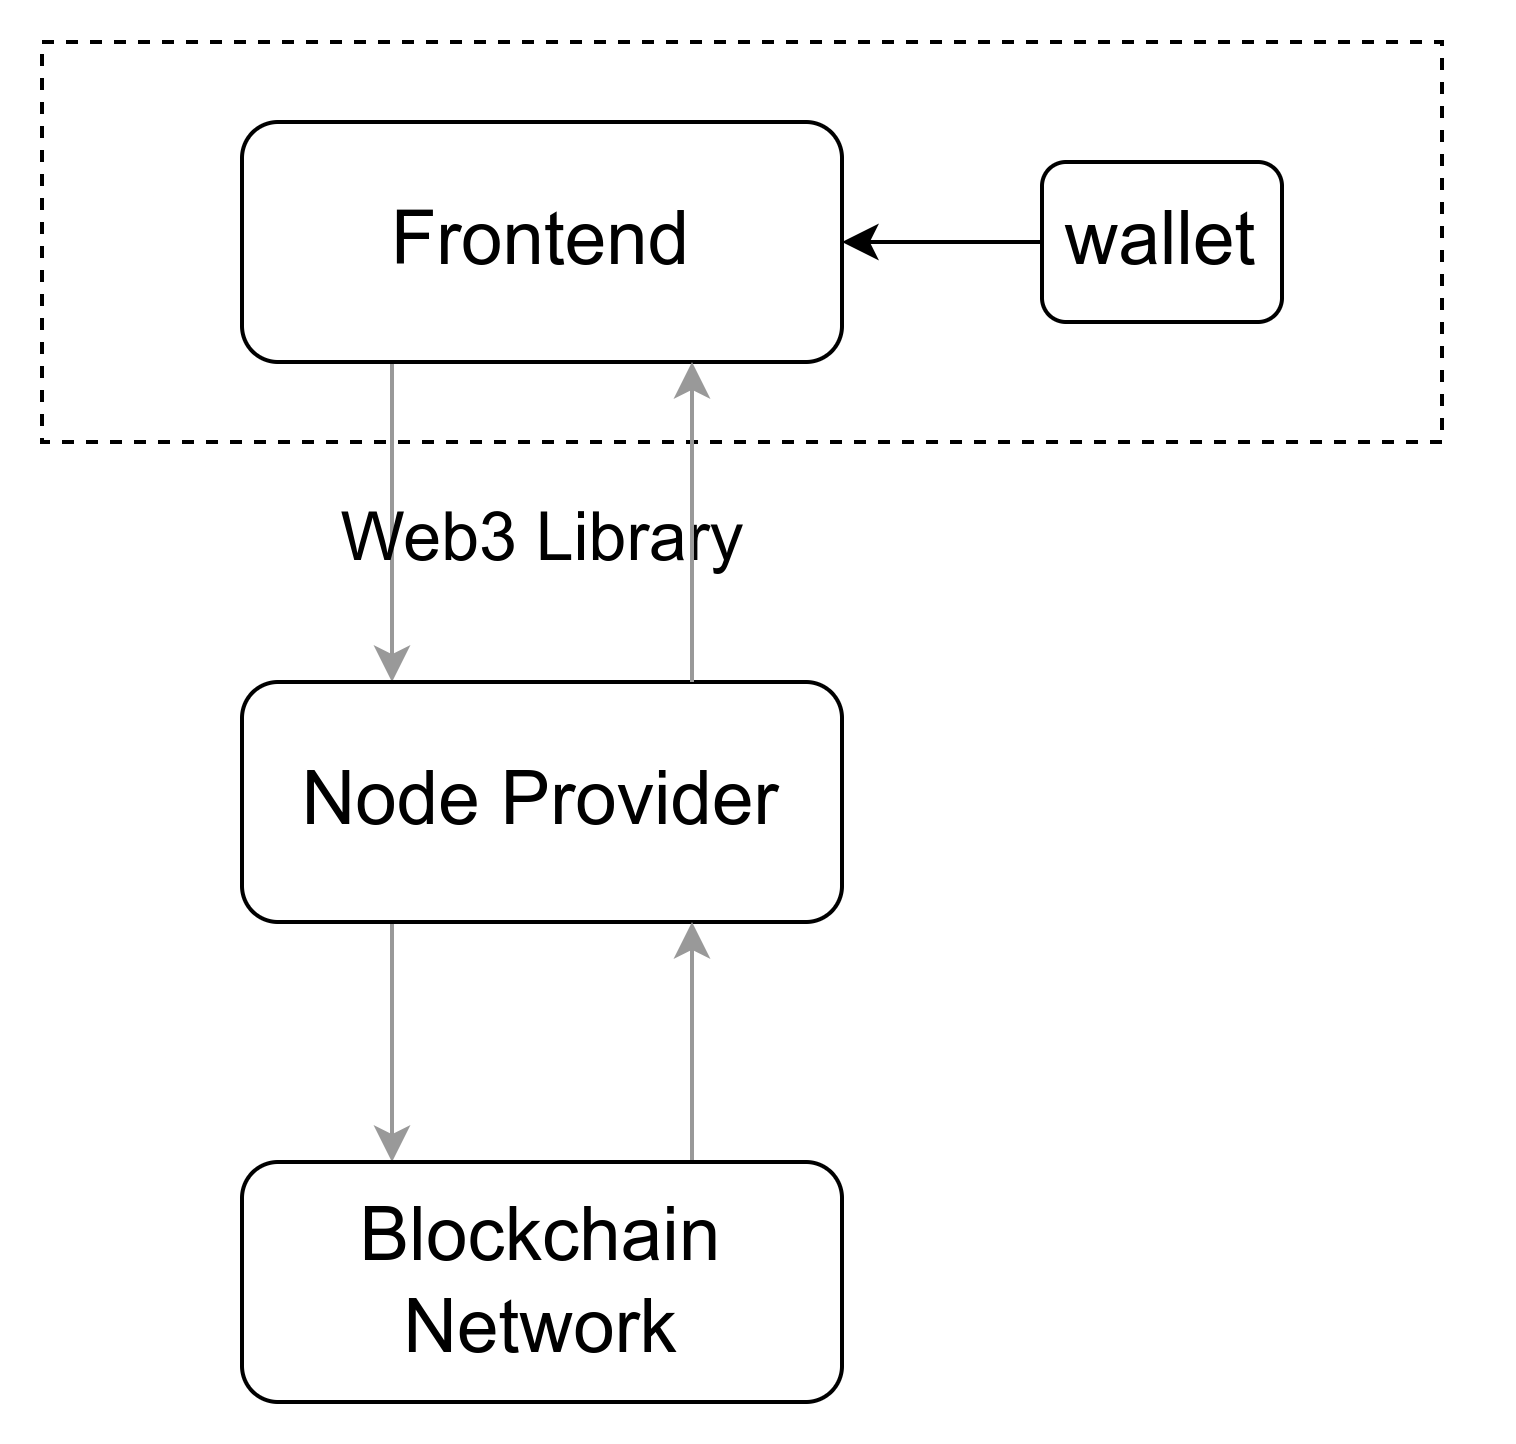
\includegraphics[width=0.6\textwidth]{./images/dapp_components}
	\caption{Basic Dapp Architecture.}
	\label{fig:dapp_components}
\end{figure}

\begin{description}		
	\item \textbf{Frontend and wallet provider}: It enables the users to interact with the smart contracts through interactive graphical components such as buttons, and icons, among others. Like web applications, this user interface runs on any browser.
	\item \textbf{Node or Node Provider}: Enables communication with the blockchain i.e. reading data or sending transactions. A node will broadcast the transactions and miners will validate the new states that the transactions can produce. Everyone can run a node. Nonetheless, because of the difficulty and costs that running a node could have, Dapps usually rely on a third-party service or Node provider. Every Ethereum client or Node provider implements a JSON-RPC\cite{json_rpc} Specification with a uniform set of methods.
	\item \textbf{The Blockchain Network}: With the smart contracts that the application will use, the EVM that runs these smart contracts, and the blockchain that stores the states and data produced by the execution of these smart contracts.
\end{description}

Furthermore, the Comunication with the Node provider is done using web3 libraries such as ethers.js\cite{ethersjs} or web3.py\cite{web3py}.
%%%%% Chapter
\chapter{Decentralized Finance (DeFi)} \label{ch:defi}
Decentralized finance or DeFi\cite{article:cefidefi}\cite{article:defi} refers to a set of decentralized applications and protocols that are focused on financial services. The term finance\cite{wiki:Finance} involves the creation, and management of money, in traditional finance systems this is done by financial institutions\cite{wiki:Financial_institution}, which emit, buy and sell financial instruments\cite{wiki:Financial_instrument} on financial markets\cite{wiki:Financial_market}, all regulated by Laws. In DeFi,  these practices and processes are determined by protocols that rely on smart contracts, which means Defi is an open, permissionless, and composable stack of protocols built on top of a permissionless blockchain such as Ethereum~\ref{sec:eth}. 
\begin{figure}[htp]
	\centering
	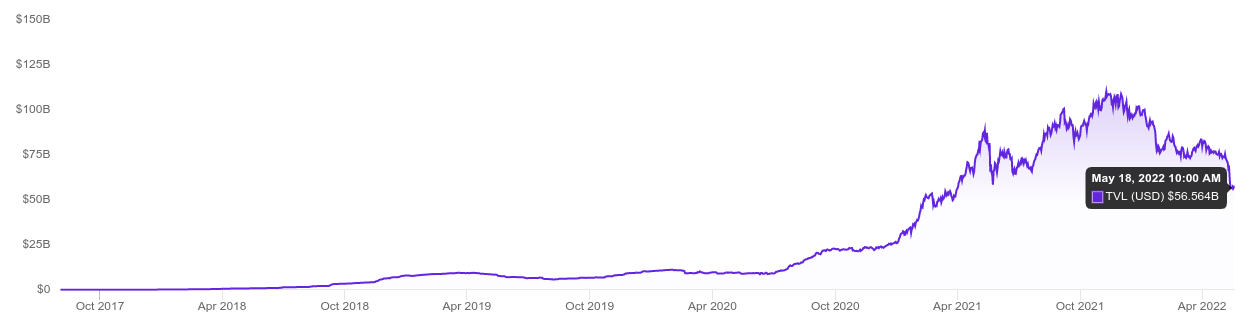
\includegraphics[width=1\textwidth]{./images/tvl}
	\caption{Total Value Locked (USD)\cite{defipulse}}
	\label{fig:tvl}
\end{figure}

DeFi offers a wide variety of financial services. For example lending and borrowing of crypto-assets, exchange of crypto assets, stable currencies, and investments oportunities, among others. Unlike traditional financial systems, is open to anyone who has internet access, users have total control of their assets and Markets are always open. Furthermore, DeFi has gained a lot of traction in the past years and according to Defipulse\cite{defipulse}, at the moment of writing this Thesis, the total locked value or TVL (held by smart contracts) in all the DeFi applications and protocols is \$58.56B~\ref{fig:tvl}, being the Maker Protocol~\ref{sec:maker}, the Aave Protocol~\ref{sec:aave}, adn he Uniswap Exchange\cite{uniswap}, the three relevant DeFi protocols of the space with $\$14.52$B, $\$8.38$B and $\$7.04$B of TVL respectively. 

\section{Maker Protocol}\label{sec:maker}
One essential piece of DeFi is stable coins or stable cryptocurrencies, and DAI~\ref{sec:dai}  is one of the most popular stable coins in the space with a market cap of \$6.5B\cite{stablecoinsmarket} at the moment of writing. Stable coins are cryptocurrencies pegged to a predetermined value, usually to the USD value. It enables DeFi users to access more traditional assets, avoiding the natural volatility of crypto assets at the current moment. In addition, due to the high demand for stable coins in the DeFi space, users can also earn interest on their stablecoins by providing liquidity into lending pools of different protocols such as Aave~\ref{sec:aave} or Compound\cite{compound}.

The Maker Protocol\cite{maker} is an open-source project built on Ethereum that enables users to generate the stable coin Dai~\ref{sec:dai}. Wich is collateral backed by different crypto assets authorized by the MakerDao, a decentralized autonomous organization (DAO)\cite{wiki:Dao}, made up of all the Maker governance token (MKR) holders. The MKR token is an ERC20 token~\ref{sec:tokens} that enables dao participants to vote on different changes or improvements to the Maker protocol.


\subsubsection{DAI}\label{sec:dai}
DAI\cite{makerDAI} is the main product of the Maker Protocol. DAI is an ERC20 token~\ref{sec:tokens},  pegged to the USD value and fully backed by different crypto assets, approved by the MakerDao, such as ETH~\ref{sec:gas}. DAI can be generated by depositing any accepted collateral crypto asset into the Maker Vaults. In short, the Maker Vaults are a set of smart contracts~\ref{sec:sc} that lock the deposited asset and generate DAI (let the user borrow DAI). The generated DAI is destroyed by the vault when the generated DAI is repaid to the Vault. Vaults are overcollateralized, for instance, at the time of writing, the Maker ETH-C Vault has a minimum collateral ratio of 170\%\cite{oasisapp}, meaning that for every \$170 of ETH deposit in the Vault a maximum of 100 DAI can be generated.

\section{Aave Protocol}\label{sec:aave}
Aave\cite{aaveV1}\cite{aaveV2}\cite{aaveV3} is a DeFi liquidity protocol that enables users to lend and borrow crypto assets. Aave was first deployed on the Ethereum network, however, at the moment of writing, Aave has expanded to other EVM-based blockchain and Layer 2 scaling solutions such as  Polygon\cite{polygon}, Avalanche\cite{avax}, Fanton\cite{fanton}, and Arbitrum\cite{arbitrum}, among many others.

Using Aave, users that supply liquidity to the protocol (lenders) earn interest on their deposited assets, and borrowers are able to borrow crypto assets after depositing collateral to the pool contract. The interest rate for users (borrowers and lenders) is decided algorithmically based on the reserves available in the pool. The reserves are the multiple currencies deposited on the pool expressed in ETH value and defined as \textit{total liquidity}. Lenders can deposit into these reserves to earn interests and Borrowers can borrow from the reserves after making a deposit, locking a greater value as collateral for the borrowed funds. Only specific low-risk crypto assets are configured as collateral. A user will be able to borrow a maximum amount depending on the Loan-To-Value (LTV) of the desired asset reserve. For instance, if the LTV value of a given asset is  60\%, for every 1 ETH value of collateral deposited, a user can borrow a maximum of 0.6 ETH value of the desired asset reserve.

\subsubsection{Interest rates}
 As mentioned in the last paragraph, for lenders and borrowers the interest rate is determined by the use of the status of the specific reserve. For \textbf{lenders}, the interest rate depends on  the \textit{current liquidity rate}: \[ R_{t} = R_{o}U \]

Where $ R_{o} $ is the overall borrow rate of the reserve defined as follows:
\begin{equation}
	R_{o} = 
	\left\{\begin{matrix}
		&  0~~if~~B_{t}=0\\ 
		& \frac{B_{v}R_{v}+ B_{s}R_{sa}}{B_{t}}~~if~~B_{t} > 0
	\end{matrix}\right.
\end{equation}
With the total amount of borrowed liquidity $B_{t} $ (\textit{total borrows}), expressed as the sum of the total stable borrows plus  the total variable borrows :
\[ B_{t} = B_{s}+B_{v} \]
The $R_{v}$\cite{aaveV1RV} is the \textit{variable borrow rate} and $R_{sa}$\cite{aaveV1RS} is the \textit{average stable rate}. 
And $ U $ is the \textit{utilization rate}, wich is the representation of the utilization of the deposited assets, defined as follows:
\begin{equation}
	U = 
	\left\{\begin{matrix}
		&  0~~if~~L_{t}=0\\ 
		& \frac{B_{t}}{L_{t}}~~if~~L_{t} > 0
	\end{matrix}\right.
\end{equation}
Where $L_{t}$  is the \textit{total liquidity} available in the reserve.

%%%%% Chapter
\chapter{Application Requirements} \label{ch:appreq}
This Chapter describes the application requirements based on ISO/IEC/IEEE 29148:2018\cite{iso} Software Requirements Specification standard.

\textbf{Project}: Thesis.
\section{Introduction}
\subsection{Purpose}
The main purpose of this Chapter is to provide a detailed description of the Decentralized application developed for this Thesis. 
\subsection{Scope}
Requirements for a decentralized application that can provide
permissionless financial services using an evm based blockchain.

The minimum viable functionality that the application shall offer the users are:
\begin{itemize}
	\item Sign in with the metamask wallet.
	\item See which tokens can be deposited.
	\item Using Aave: Deposit cryptoassets and earn interest. 
	\item Using Aave: Withdrawal of deposited assets.
\end{itemize}
The application runs online; its frontend may not be decentralized, but its backend runs on top of an EVM-based blockchain such as Polygon Testnet or Mainnet.
\subsection{Product Perspective}
\subsubsection{Interface}
The application runs in the latest version of Chrome, Firefox, Brave browsers on Windows, Linux and Mac.

\section{Requirements}
\subsection{Functional}
\subsubsection{Login}
[Thesis-SRS-01] The application shall allow users to login using the Metamask\cite{wiki:MetaMask} wallet.

[Thesis-SRS-02]  If the wallet is set with another network, the application should let the user change to the application network with just one button click.

[Thesis-SRS-03] The application shall display the user balance of the supported assets.

[Thesis-SRS-04] The application shall display the user balance of deposit assets and earnings.

[Thesis-SRS-05] The application shall display the interest rates for the supported assets.
\subsubsection{Deposit}
[Thesis-SRS-06] The application shall allow users to deposit Ether to earn interest.

[Thesis-SRS-07] The application shall allow users to deposit DAI to earn interest.

[Thesis-SRS-08] The application shall convert Ether to Weth, because the protocol only accepts Ether in the form of ERC20, i.e. Weth.

[Thesis-SRS-9] The application shall display the user balance after any deposit transaction.

\subsubsection{Withdrawal}
[Thesis-SRS-10] The application shall allow users to withdraw deposited cryptoassets.

[Thesis-SRS-11] The application shall display the user balance after any withdrawal transaction.

\subsection{Nonfunctional}
\subsubsection{Login}
[Thesis-SRS-12] While not logged in, the application should display the available assets to be deposited and its interest rates. 
\subsubsection{Deposit}
[Thesis-SRS-13] The application should display a notification after any deposit transaction.
\subsubsection{Withdrawal}
[Thesis-SRS-14] The application should display a notification after any withdrawal transaction.
\subsubsection{Performance}
[Thesis-SRS-15] The transaction cost should be minimized by using the Polygon network.

\newpage
\section{Use Case}
The following use case diagram describes the minimum functionality that the application shall have.

\begin{figure}[htp]
	\centering
	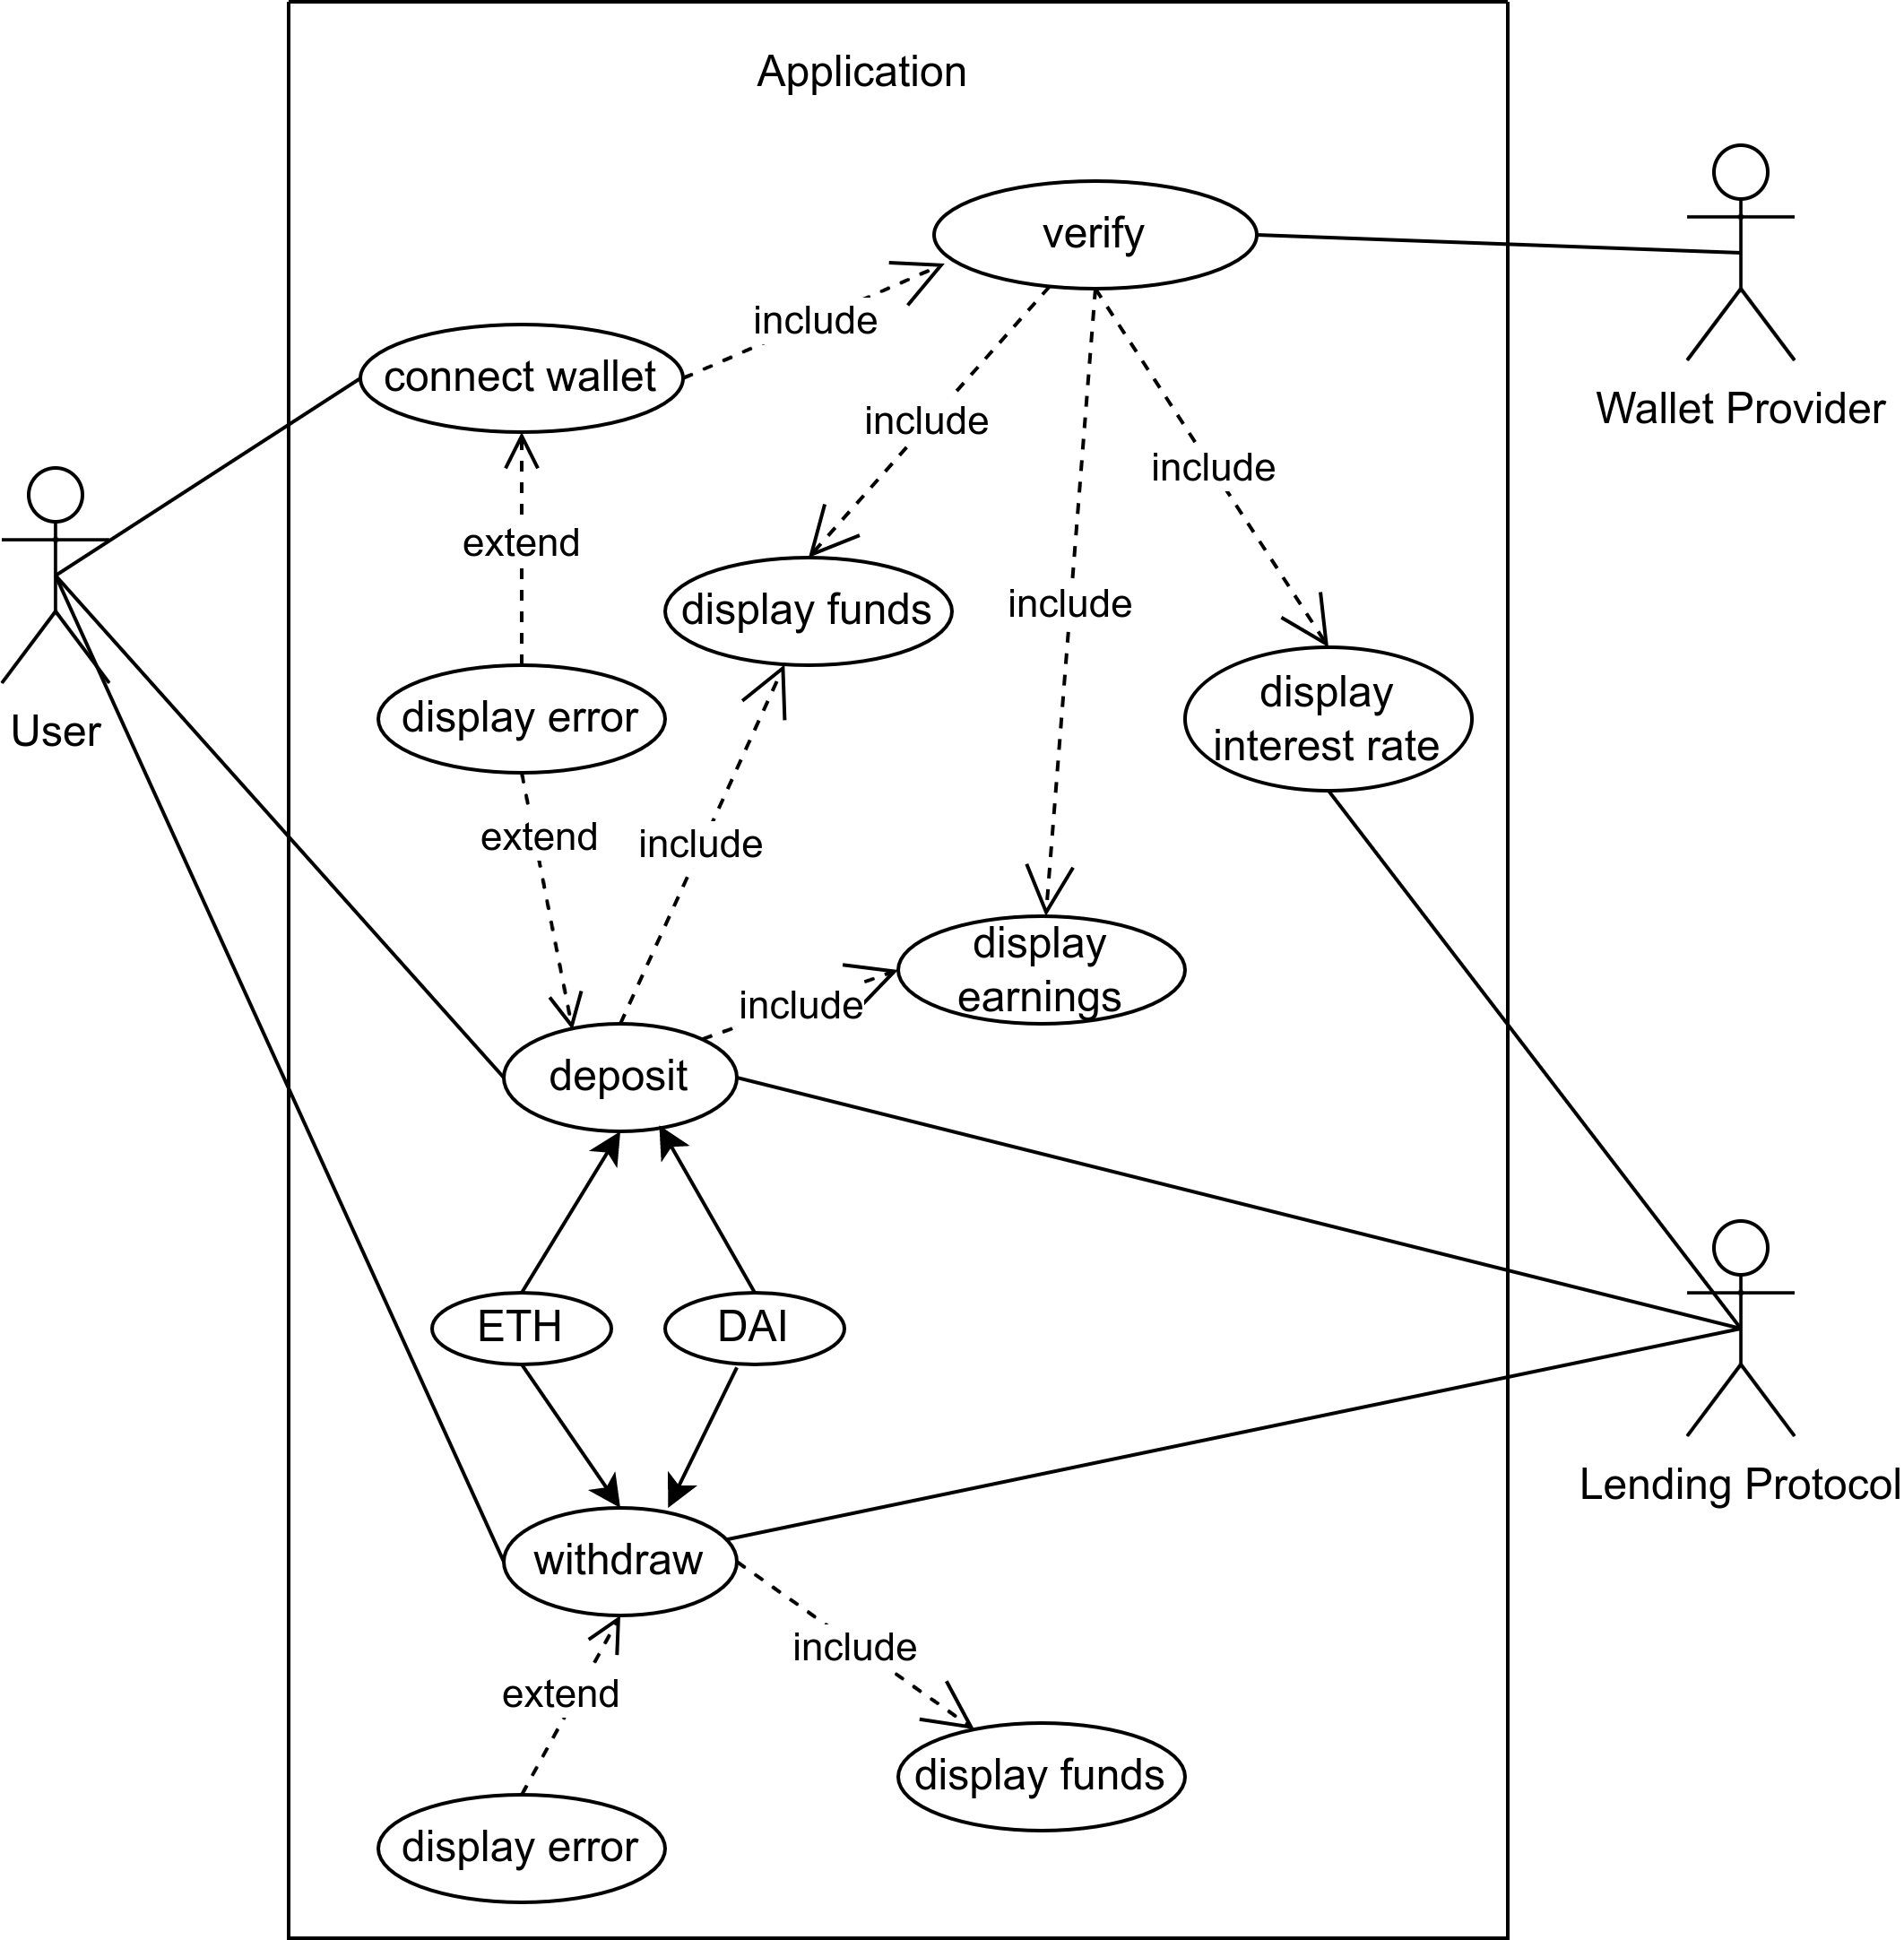
\includegraphics[width=1\textwidth]{./images/USECASE-mvp}
	\caption{Use Case Diagram: Minimum Viable Product.}
	\label{fig:usecase-mvp}
\end{figure}
\newpage
%If the development process goes well and there is enough time, the application should add %more functionalities as illustrated in the following use case diagram. The requirement %document/chapter\cite{ch:appreq} should also be updated.
%\begin{figure}[htp]
%	\centering
%	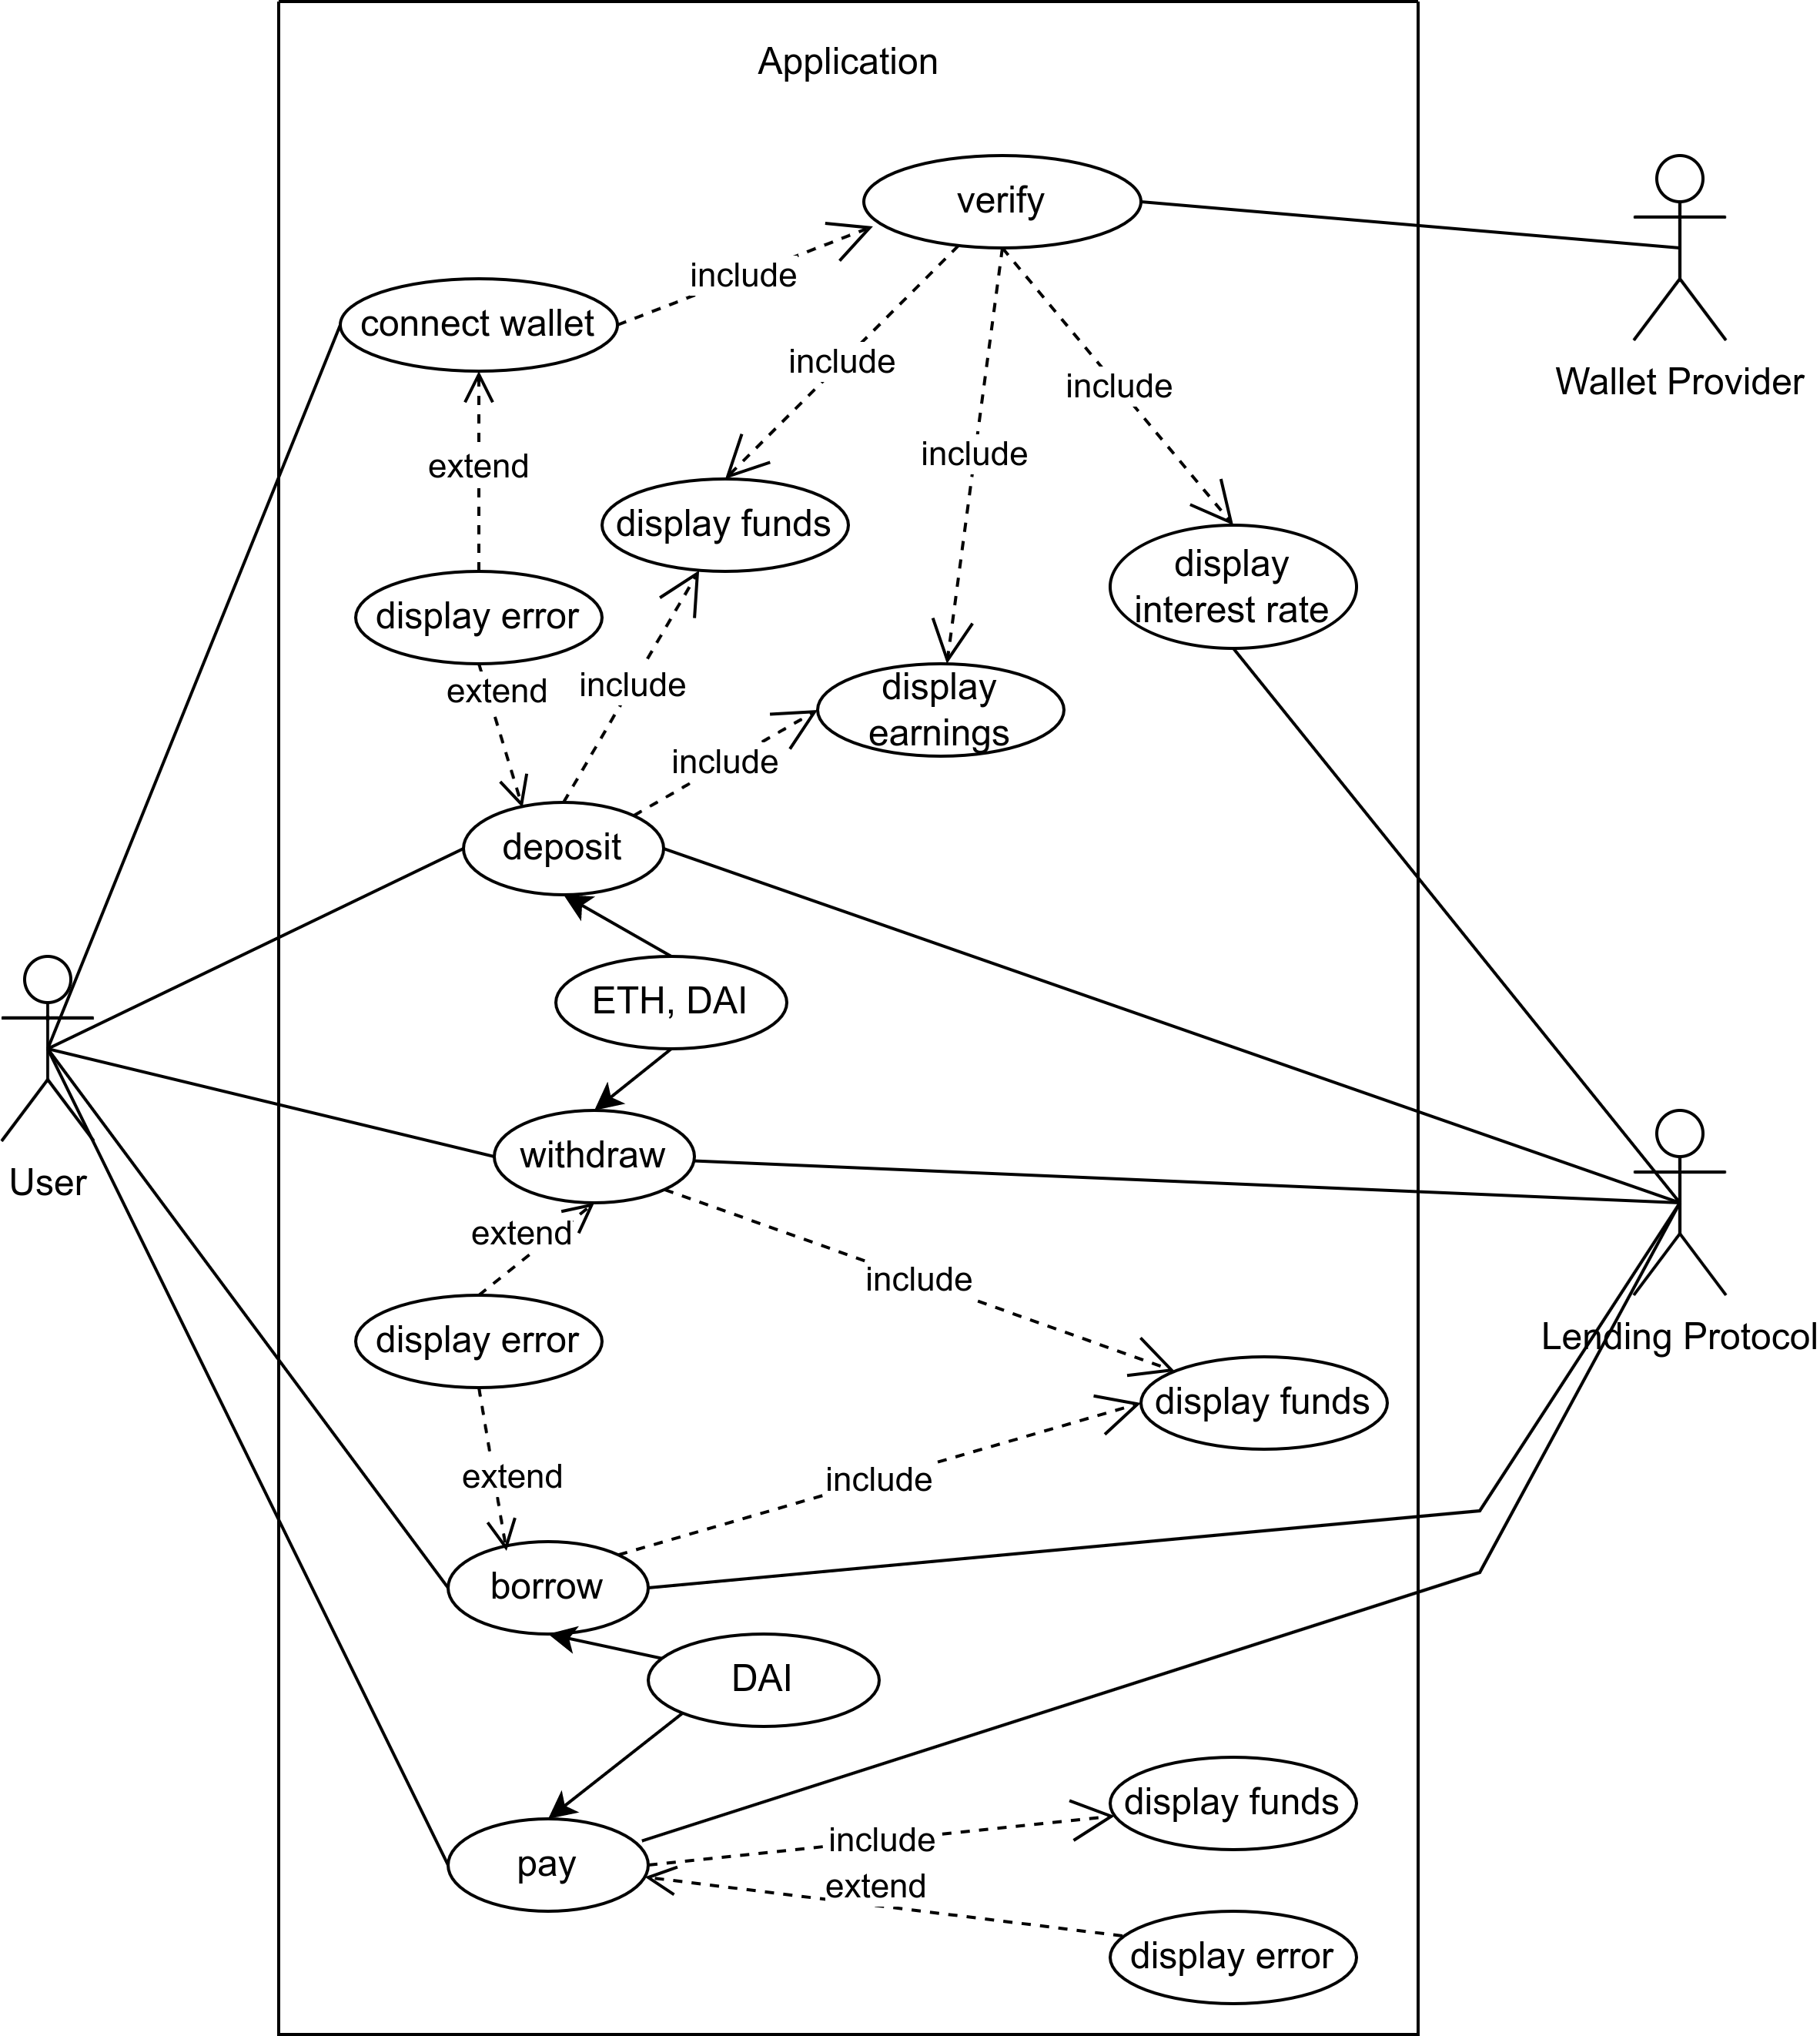
\includegraphics[width=0.97\textwidth]{./images/USECASE-full_nofl}
%	\caption{Use Case Diagram: Expected Application Functionality.}
%	\label{fig:usecase-mvp}
%\end{figure}


%%%%% Chapter
\chapter{Implementation and testing} \label{ch:impl}
%\section{Defining the tech stack}
\section{Node Provider}
\subsection{Alchemy}
\section{Intearction with the smart contracts: Backend}
\subsection{Web3.py: Brownie}
\subsection{Testing: pytest}
\section{Interaction with the users: Frontend}
\subsection{Next.js}
\subsection{Ethers.js: web3 react hocks}
\subsection{Testing: mochajs?}
%%%%%
%%%%% Chapter
\chapter{Conclusion and future work} \label{ch:conclusion}
\newpage

\bibliographystyle{plain} % Literaturverzeichnis
\begin{btSect}{thesis} % mit bibtopic Quellen trennen
\section*{Bibliography}
\btPrintCited
\end{btSect}
\begin{btSect}{online}
\section*{Online Sources}
\btPrintCited
\end{btSect}
% dann mit "bibtex thesis1" und "bibtex thesis2" arbeiten

\end{document}
;;; Local Variables:
;;; ispell-local-dictionary: "de_DE-neu"
;;; End:
